\documentclass{crypto-exercise}
\usepackage{amsthm}
\usepackage{tikz}
\author{Sven Laur}
\contributor{}
\editor{}
\tags{false positives, false negatives, statistical distance}


\begin{document}
\begin{exercise}{Complete constellation of distinguishers}
For any distinguisher $\AD$ and two distributions $\XXX_0$ and $\XXX_1$, define the false-positive rate
\begin{align*}
\alpha(\AD)=\pr{x\gets\XXX_0: \AD(x)=1}\enspace\phantom{.}
\end{align*}
and the false‑negative rate 
\begin{align*}
\beta(\AD)=\pr{x\gets\XXX_1: \AD(x)=0}\enspace.
\end{align*}
Then it is straightforward to prove the following inequality 
\begin{align}\label{ineq}
1-\SD_x(\XXX_0,\XXX_1)\leq \alpha(\AD) +\beta(\AD)\leq 1+\SD_x(\XXX_0,\XXX_1)
\end{align}
Let us define distributions $\mathcal{X}_0$ and $\mathcal{X}_1$ over the set $\{0,1,\ldots, 9\}$ such that  for any $i\in\set{0,\ldots, 9}:$
\begin{align*}
\pr{x\gets \XXX_0: x=i}&=\frac{i}{45}\enspace.\\
\pr{x\gets \XXX_1: x=i}&=\frac{9-i}{45}\enspace.
\end{align*}
Compute the statistical distance between the distributions $\XXX_0$ and $\XXX_1$ and place all non-trivial distinguishers (a distinguisher that is not expressable as a mixture of two other distinguishers) on the following figure  
\begin{center}
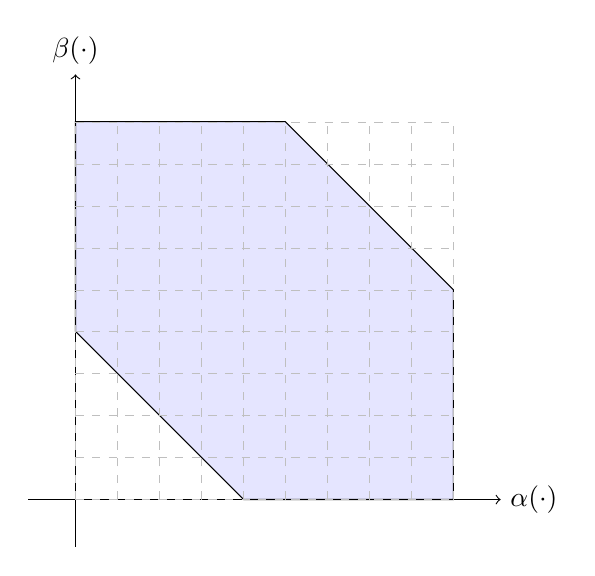
\begin{tikzpicture}[scale=1.2]
    % Axes
    \draw[->] (-0.5,0) -- (4.5,0) node[right] {$\alpha(\cdot)$};
    \draw[->] (0,-0.5) -- (0,4.5) node[above] {$\beta(\cdot)$};


    \fill[fill=blue!10, draw=black] (0,4) -- (0,1.78) -- (1.78,0) -- (4,0) -- (4,2.22) --(2.22, 4) -- cycle;

    % Grid (optional)
    \draw[help lines, dashed, gray!50, step=0.444cm] (0,0) grid (4,4);

\end{tikzpicture}
\end{center}



\end{exercise}


\begin{solution}
\end{solution}

\end{document}

